%
% $RCSfile: input_output_and_rules.tex,v $
%
% Copyright (C) 2002-2008. Christian Heller.
%
% Permission is granted to copy, distribute and/or modify this document
% under the terms of the GNU Free Documentation License, Version 1.1 or
% any later version published by the Free Software Foundation; with no
% Invariant Sections, with no Front-Cover Texts and with no Back-Cover
% Texts. A copy of the license is included in the section entitled
% "GNU Free Documentation License".
%
% http://www.cybop.net
% - Cybernetics Oriented Programming -
%
% http://www.resmedicinae.org
% - Information in Medicine -
%
% Version: $Revision: 1.1 $ $Date: 2008-08-19 20:41:07 $ $Author: christian $
% Authors: Christian Heller <christian.heller@tuxtax.de>
%

\subsubsection{Input/Output and Rules}
\label{input_output_and_rules_heading}
\index{Data Structure}
\index{Enterprise Resource Planning System}
\index{ERP}
\index{Knowledge Model}
\index{Steady State}
\index{Converter containing Rules}
\index{Black Box}
\index{Logic Model}
\index{State Model}
\index{Information Flow}

In order to process data correctly, a system needs to know about their
\emph{Structure}. Software systems work with data belonging to some knowledge
model. Chapter \ref{knowledge_schema_heading} demonstrated how knowledge can be
modelled. Many applications keep their knowledge in special data files. Others,
such as \emph{Enterprise Resource Planning} (ERP) systems, retrieve their data
from a database. Even systems claiming to do nothing than pure data processing,
possibly using one operation only, rely on simple knowledge models, for at
least their \emph{Input/Output} (i/o) data.

Living systems rely on constantly exchanging information, energy, nutrients and
excretion products with their environment; they are never in a stationary, but
always in a \emph{Steady State}. A biological cell, for example, has inputs and
outputs and reacts in a certain manner which, after \cite{sengbusch}, is best
modelled with a \emph{Converter} containing \emph{Rules}, and treated as black
box. The cell's characteristic behaviour results from the way it relates inputs
to outputs.

\begin{figure}[ht]
    \begin{center}
        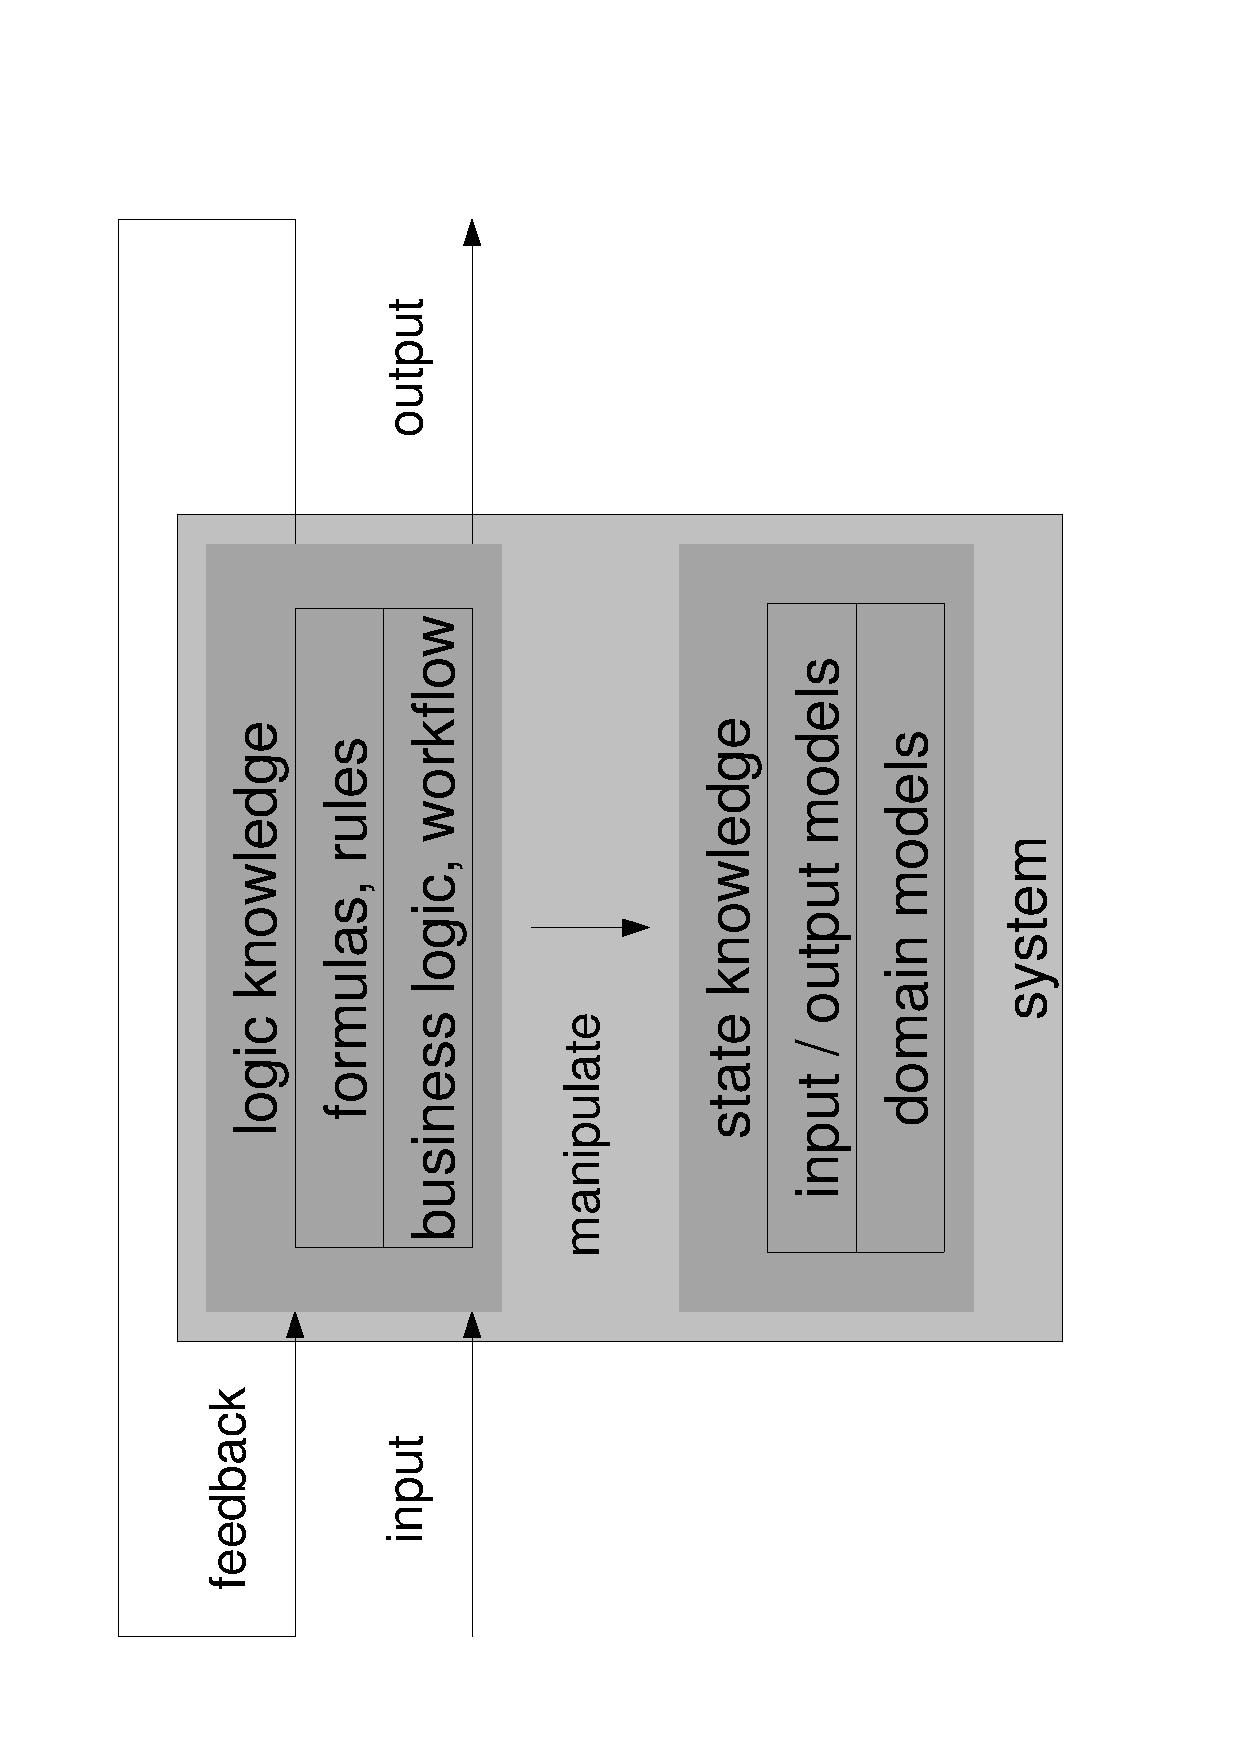
\includegraphics[scale=0.3,angle=-90]{graphic/manipulation.pdf}
        \caption{Logic translates between Input-, Domain- and Output States}
        \label{manipulation_figure}
    \end{center}
\end{figure}

Whilst figure \ref{blackbox_figure} illustrated the i/o flow of a system from
an \emph{outside} view, figure \ref{manipulation_figure} also considers the
state- and logic knowledge situated \emph{inside} a system. The arrow
indicating the information flow is directed from \emph{Logic-} towards
\emph{State} models, because the former manipulate the latter.
